\section{Credit Distribution and Distribution Strategies}
\label{section:distribution_strategies}

\subsection{Data Credit and Data Credit Distribution}
Given a database instance $I$, a \emph{recipient of credit} corresponds to a unit of information within the same database. In the case of relational databases, recipients may be (i) the whole database itself; (ii) a table; (iii) a tuple; (iv) an attribute.

\emph{Data credit} is a value $k \in \mathbb{R}_{>0}$ used to represent the value of a recipient in a database. 
Every recipient in a database is annotated with a given quantity of credit, as a proxy for its importance in a certain context. In this paper, we focus on tuples as recipients of credit. 

\emph{Data Credit Distributions} (DCD) considers a database instance $I$, a certain quantity of credit $k$ (here, without loss of generality, deemed to be given), and a query $Q$ producing a result set $Q(I)$.  
DCD consists of defining a function, i.e., a \emph{distribution strategy} (DS), to split credit into portions to be assigned to the tuples in $I$.

In the following, we follow the notation given by \citet{CheneyProvSurvey}: a \emph{tuple location} is defined as a tuple in one relation of $I$, tagged with its name. It is indicated with $(R, t)$, where $R$ is the relation in the database, and $t$ is the tuple in $R$. With reference to the running example, \texttt{(family, $\langle f_1$, Dopamine Receptors, gpcr$\rangle$)} is the tuple location of the first tuple in the \texttt{family} relation.  The set of all the tuple locations in $I$ is called \emph{TupleLoc}.
The following is the definition of DCD at \emph{tuple level}. We refer to the level of tuple because the credit is annotated to tuples.

\begin{definition}
    \textbf{Data Credit Distribution at tuple level} (DCD)~\citep{dosso2020data}
    \label{def:CDT}\\
    Given a database instance $I$, a query $Q$ over $I$ and the value $k \in \mathbb{R}_{>0}$, DCD is defined as the computation of the function $f_{I, Q} : TupleLoc \times \mathbb{R}_{> 0} \rightarrow \mathbb{R}_{\geq0}$ such that $f_{I,Q}(t, k)=h$ where $0 \leq h \leq k$ and $\sum_{t \in TupleLoc}f_{I, Q}(t, k) = k$.
\end{definition}

As we see, the DS is a function that annotates each tuple in the database with a real value, which is a fraction of the given quantity $k$. The only constraint is that the sum of the credit fractions annotation the tuples must be $k$ (i.e. no credit is generated nor destroyed during the distribution).
Given $I$ and $Q$, many different DS may be defined as long as they sum up to $k$. We use the information provided by data provenance to define sensible functions that take into account the issued query. 

\subsection{A Lineage-based Distribution Strategy}
With the information provided by the lineage, we defined the following DS:

\begin{definition}{Lineage-based Distribution Strategy}~\citep{dosso2020data}
    \label{def:lineage_ds}\\
    Let $I$ be a database instance, $Q$ a query over $I$, $o \in Q(I)$ an output tuple and $k$ the credit associated to $o$.
    Let $L$ be the lineage of $o$ and $t$ be a generic tuple in $I$, then $t$ receives a credit equal to:
    \begin{equation*}
        f_{I, Q}(t, k) =  \begin{cases}
         0 & \mbox{if $t \notin L$} \\
            \frac{k}{|L|} & \mbox{if $t \in L$}
        \end{cases}
    \end{equation*}
\end{definition}

%It is trivial to see how this is actually a Distribution Strategy since the sum of all the values assigned by the set of functions returns exactly the value $k$:
%
%\[
%\begin{array}{ll}
%    \sum_{t \in I}f(t, k) & = \sum_{t \notin L}f(t, k) + \sum_{t \in L}f(t, k)\\
%    & = 0 + \sum_{t \in L}\frac{k}{|L|}  \\
%     & = \frac{k}{|L|}\sum_{t \in L}1 \\
%     & = k
%\end{array}{}
%\]

The DS is defined for one tuple of the output. Therefore, to perform credit distribution for a whole set of output tuples, it is necessary to first divide the credit to each tuple in the output and then compute the distribution for each one of them.
In this paper, we assume that each output tuple carries credit equal to 1. 
This lineage-based DS distributes credit only among tuples that have a role, whichever it is, in creating $o$ by the query $Q$. Each of them receives an equal share of the credit. The more the tuples in a lineage set, the less the credit every single tuple receives. 


As an example, consider the output tuples of Table \ref{table:result}.
Each output tuple has credit $k = 1$.
The lineage of the first tuple is the set $\{f_1, c2f_1, c_1, c2f_2, c_2\}$. Therefore, each tuple in this set receives credit $1/5$. The other tuples of the database receive zero credit.
The lineage of the second output tuple is $\{ f_4, c2f_4, c_1\}$, therefore each of these tuples receives credit $1/3$.

At the end of the process, tuples $f_1, c2f_2, c_2$ receive credit $1/5$ each, tuples $f_4$ and $c2f_4$ receive $1/3$, while tuple $c_1$ receive $8/15$.  
Suppose one tuple appears in more than one lineage set. In that case, it will accumulate credit from the distribution associated with each one of these sets, implying its more significant relevance in the context of the considered query, as is the case with $c_1$ in this example.
 
Not all of the tuples of the lineage of $o_1$ are necessary at the same time for the generation of the tuple. 
If the database only had the set of  tuples $\{f_1, c2f_1, c_1\}$ or the set $\{f_1, c2f_2, c_2\}$, its existence would still be guaranteed. 
In other words, only one among the couples of tuples $\langle c2f_1, c_1 \rangle$ and $\langle c2f_2, c_2 \rangle$ is required, while $f_1$ is always needed. 
One could argue that it would be fairer for $f_1$ to receive more credit than the other four tuples, given its role in producing $o_1$.  

This highlights one limitation of the DS based on lineage: while able to find all and only the relevant tuples of the output, it cannot distinguish the \emph{importance} of tuples in the query computations. 
This information could be incorporated in the definition of a DS to distribute credit based on the actual role that tuples play in the computation. 

For this reason, we present in this paper more sophisticated forms of Distribution Strategies, based on the other two provenances discussed above.

\subsection{A Why-Provenance-Based Distribution Strategy}

 \begin{definition}{Why-Provenance-based Distribution Strategy}\\
        \label{def:why_distribution}
    Let $I$ be a database instance, $Q$ a query over $I$, $o \in Q(I)$ an output tuple and $k$ the total credit associated to $o$. Let $t$ be a generic tuple in $I$.
    Let us call $\mathcal{W} = Why(Q, I, o)$ the witness basis of $o$ according to $Q$ and $I$, where $W \in \mathcal{W}$ is a generic witness. 
    Let us call $\gamma(\mathcal{W}, t): (\mathcal{W}, t) \mapsto \mathcal{P}(\mathcal{P}(TupleLoc))$ the function that returns the set 
    $\{W \in \mathcal{W} : t \in W\}$.
    % of all the witnesses $W \in \mathcal{W}$ such that $t \in W$. 
    The tuple $t$ receives a credit equal to:
    \begin{equation*}
        f_{I, Q}(t, k) =
            \frac{k}{|\mathcal{W}|}\sum_{W \in \gamma(\mathcal{W}, t)}\frac{1}{|W|}
    \end{equation*}
\end{definition}
%We now prove that this set of functions is a Distribution Strategy. As we can see, with abuse of language we use $t \notin \mathcal{W}$ to indicate the input tuples $t$ that are not present in any witness.
%\[
%\begin{array}{rl}
%\sum_{t \in I}f_{I, Q}(t, k) & = \sum_{t \notin \mathcal{W}}f_{I, Q}(t, k) + \sum_{t \in \mathcal{W}} f_(I, Q)(t, k)\\
%                    & = 0 + \frac{k}{|\mathcal{W}|}\left[\sum_{W \in  \mathcal{W}} \left(\sum_{t \in W}\frac{1}{|W|}\right)\right]\\
%                    & \frac{k}{|\mathcal{W}|}\sum_{W \in  \mathcal{W}} 1 \\
%                    & = \frac{k}{|\mathcal{W}|}|\mathcal{W}|\\
%                    & = k
%\end{array}
%\]
This strategy first equally distributes the credit among the witnesses of the witness basis then, successively, it further equally divides the credit among the tuples in a witness. 
Since one tuple may appear in more than one witness, it will receive more than one portion of credit from the same distribution. 

\begin{figure}[]
\centering
  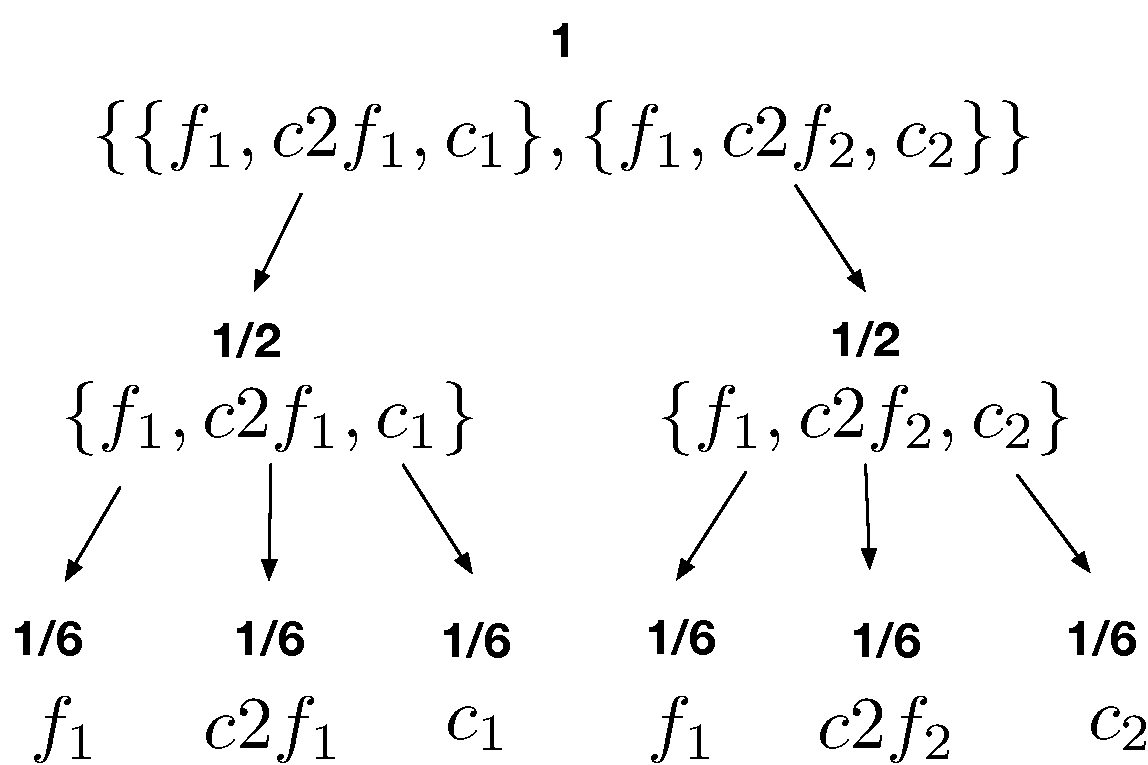
\includegraphics[width=.45\textwidth]{figures/why_distribution}
  \caption{Exemplification of the distribution of credit through the why-provenance based DS for tuple $o_1$.}
  \label{figure:why_prov_distribution}
\end{figure}

Figure \ref{figure:why_prov_distribution} represents the distribution of credit with this DS with the why-provenance of tuple $o_1$.
The credit is first divided among the two witnesses, that both receive credit $1/2$. 
The credit is then further divided among the tuples in each witness. Each tuple in each witness receives $1/6$ of credit. At the end of the distribution, $f_1$ receives a cumulative total credit of $1/3$, the other tuples receive $1/6$ each.
This distribution better reflects the role of $f_1$ in the generation of $o_1$ since, as we discussed, it is the only mandatory tuple for the production of the output, while we need only one of the two other couples of tuples to get the result. 

From this example, it is immediately evident how why-provenance can better reward the tuples depending on their role. Tuples that appear in more than one witness are rewarded more than others. This means that tuples that are more important to the generation of the output, since they are used more by the query, are rewarded more than tuples that are ``interchangeable'' with others. 

\subsection{A How-Provenance Based Distribution Strategy}
\label{section:how_prov_distr_tuples}
The how-provenance conveys more information than the why-provenance since it does not only capture what tuples are relevant to the output and in which combination, but also how they are used. To define the Distribution Strategy based on the how-provenance, we first need some other preliminary definitions.

Consider the provenance polynomial $\mathcal{H} = H(Q, I, o)$ of a tuple $o$. We define: 
\begin{enumerate}
	\item $c(\mathcal{H}) = n$ the function $c: \mathbb{N}[TupleLoc] \mapsto \mathbb{N}$ that, given a polynomial, returns the sum of its coefficients;
	\item $c(M)$ the function $c: \mathcal{M} \mapsto \mathbb{N}$ that, given a monomial $M$, returns the sum of its exponents (with $\mathcal{M} \subset \mathbb{N}[TupleLoc]$ such that $\mathcal{M}$  is made only by the monomials $M$ in $\mathbb{N}[TupleLoc]$); 
	\item $e(t, M)$ the function $e: TupleLoc \times \mathcal{M} \mapsto \mathbb{N}$ that, given in input a tagged tuple and a monomial, returns the exponent of that tuple inside the monomial;
	\item $mc(M)$ the function $mc: \mathcal{M} \mapsto \mathbb{N}$ that, given in input one monomial, returns its coefficient;
	\item $\gamma(t, \mathcal{H})$ the function $\gamma: TupleLoc \times \mathbb{N}[TupleLoc] \mapsto \mathcal{M}$ that, given a tuple $t$ and a provenance polyomial $\mathcal{H}$, returns the (possibly empty) set of monomials $M$ in $\mathcal{H}$ such that $t$ appears in $M$.
\end{enumerate}

\begin{definition}{\textbf{How-Provenance-Based Distribution Strategy}}
    \label{def:how_distribution}\\
    Let $I$ be a database instance, $Q$ a query over $I$, $o \in Q(I)$ an output tuple and $k$ the total credit associated to $o$. Let also $t$ be a generic tuple in $I$. The credit given to $t$ is:
    \[
    f_{I, Q}(t, k) = \frac{k}{c(\mathcal{H})} \sum_{M \in \gamma(t, \mathcal{H})} mc(M) \frac{e(t, M)}{c(M)}
    \]
\end{definition}

%We demonstrate that this is a Distribution Strategy by considering the contributions of the single monomials one at a time in the sum. With abuse of language in the following demonstration, we write $t \in M$ to indicate one tuple $t$ appearing in the monomial $M$.
%
%\[
%\begin{array}{rl}
%\sum_{t \in I}f(t, k) & = \sum_{t | \gamma(t, \mathcal{H}) = \emptyset}f(t, k) + \sum_{t | \gamma(t, \mathcal{H}) \neq \emptyset}f(t, k) \\
%    & = 0 + \sum_{M \in l(\mathcal{H})} \left(k \cdot \frac{mc(M)}{c(\mathcal{H})} \sum_{t \in M} \left[\frac{e(t, M)}{c(M)} \right]\right)\\
%    & = \frac{k}{c(\mathcal{H})}\sum_{M \in l(\mathcal{H})} \left[ \frac{mc(M)}{c(M)} \sum_{t \in M} e(t, M)  \right] \\
%    & = \frac{k}{c(\mathcal{H})} \sum_{M \in l(\mathcal{H})} mc(M)\\
%    & = k
%\end{array}
%\]

The how-provenance-based DS first distributes the credit to the monomials of the polynomial accordingly to the weight represented by their coefficients, then to the single tuples in every monomial accordingly to the weights represented by their exponents. 

Going back to the example of Table \ref{table:result_how_prov}, consider $o_1$, that has provenance polynomial $f_1 c2f_1 c_1 + f_1 c2f_2 c_2$. The DS firstly divides the credit between the two monomials. Since the coefficients are both $1$, the credit is split in half. If they were, for example, $1$ and $2$ respectively, $1/3$ of the credit would go to the first monomial, $2/3$ to the second.  
Since in our example each variable has exponent $1$, the credit is further divided equally among the three variables. Thus, at the end of the computation, $f_1$ receives $1/3$, the other tuples receive $1/6$.
If, for example, the first monomial was $f_1^2 c2f_1 c_1$, then the portion of credit of this monomial would be divided in this way: $1/2$ to $f_1$ and $1/4$ to each of the other two tuples. 

In this specific example, the how-provenance-based distribution has the same outcome of the strategy based on why-provenance. %Consequently, one may ask if there is a significant difference between the two strategies. 
Thus, let us consider this new query \texttt{Q2}, that asks for the families of type \texttt{gpcr} that have as contributor a researcher localized in the UK from GtoPdb:
\begin{verbatim}
	Q2: SELECT DISTINCT F.name 
	FROM family as F JOIN
		(SELECT DISTINCT f.name AS name
		FROM family AS f JOIN contributor2family AS c2f ON f.id = c2f.family_id
		JOIN contributor AS c ON c2f.contributor_id = c.id
		WHERE c.country = 'UK') AS R ON F.name = R.name
	WHERE F.type = 'gpcr'
\end{verbatim}

\begin{table}[]
\centering
  \begin{tabular}{|l|c|}
  \hline
    id & name\\
    \hline
    $oxs_1$ &  Dopamine Receptors\\
    \hline
  \end{tabular}
  \begin{tabular}{c | c | c}
  	lineage & why-provenance & how-provenance   \\
  	$\{f_1, c2f_1, c_1, c2f_2, c_2\}$ & $\{\{f_1, c2f_1, c_1\}, \{f_1, c2f_2, c_2\}\}$ & $f_1(f_1 c2f_1 c_1 + f_1 c2f_2 c_2)$\\
  \end{tabular}
    \caption{Result of query \texttt{Q2} applied on the database of Table \ref{table:running_example} and its different provenances. The reported numbers are the credit distributed through the process.}
  \label{table:difference_result}
\end{table}

Table \ref{table:difference_result} presents the result, composed of one tuple, annotated with the three provenances. As can be seen, lineage and why-provenance are identical to those of the tuple $o_1$ in the previous example. 
The how-provenance is different since tuple $f_1$ is used twice: firstly, in the join of the inner query, secondly in the join of the outer query. This information is lost in the first two provenances since they are sets, but it is maintained in the how-provenance through the use of the operator `$\cdot$'.

\begin{figure}[]
  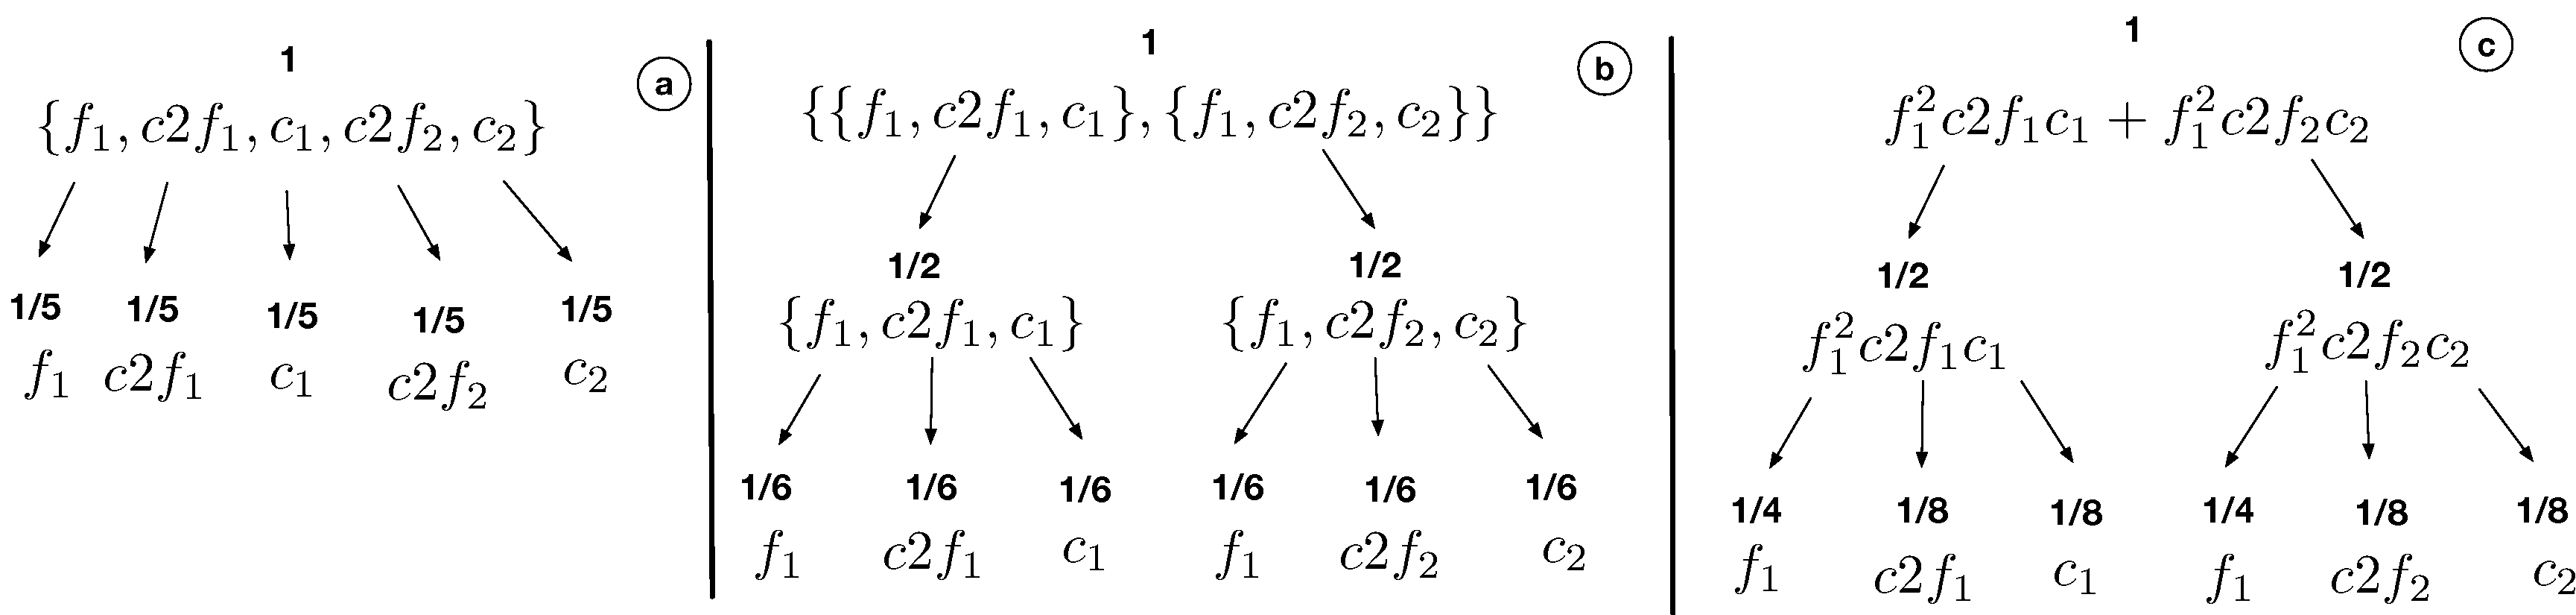
\includegraphics[width=\textwidth]{figures/how_distribution}
  \caption{Comparison of different distributions strategies from the credit of tuple $o_1$ produced by query \texttt{Q2}.}
  \label{figure:distributions_differences}
\end{figure}


Figure \ref{figure:distributions_differences} shows the differences between the three DS for the tuple $o_1$ of Table \ref{table:difference_result}. In subfigure \ref{table:difference_result}.a we used lineage, in sub-figure \ref{table:difference_result}.b we used why-provenance, and in sub-figure \ref{table:difference_result}.c we used how-provenance. 
The DS based on the provenance polynomial gives credit $1/2$ to $f_1$, and $1/8$ to the other tuples.
This is reasonable since \texttt{Q2} utilizes $f_1$ even more than \texttt{Q1}. 
The distribution based on how-provenance can reward $f_1$ more, proving that how-provenance is even more sensitive to the tuples' role in a query than why-provenance. In this case, the why-provenance is not sensible to this difference. 
This is somehow a direct consequence of the fact that, as demonstrated in \citep{howProvenanceGreen}, how-provenance is more general than why-provenance and lineage, in the sense that it contains more information. 
